\chapter[Code demonstration and validation]{Code demonstration and validation}

\section{Demonstration and Validation approach}
The SaltProc after finishing development process will be tested for several 
different \gls{MSR} concept designs. The concepts with various fuel salt 
compositions, number of salts (single- and two-fluid), neutron spectrum and 
reprocessing schemes will be investigated. In particular, demonstration 
and validation activity will be focused on \gls{TAP} \gls{MSR} which is 
promising and relatively recent concept of commercial \gls{MSR}. The results 
obtained with SaltProc python package will be compared with recent research 
efforts 
discussed in Chapter 2 of current work (see table~\ref{tab:fs_codes}). 
Table~\ref{tab:msr_concepts} 
contains tentative list of \glspl{MSR} concepts which are selected for 
demonstration and validation proposes and their principal design features. 
Finally, a compatible \textit{.JSON} database with input examples of listed 
concept models for use with the SaltProc will be released to encourage 
research efforts in online reprocessing simulations for various 
\gls{MSR} designs.
\begin{table}[!htb]
  \centering
  \caption{Tentative list of \glspl{MSR} designs selected for SaltProc 
  demonstration and validation and their principal parameters.}
  \label{tab:msr_concepts} 
  \begin{tabular}{p{0.25\textwidth} p{0.22\textwidth} p{0.22\textwidth} p{0.22\textwidth} } \toprule 
   Parameter & \gls{TAP} & \gls{MSBR} & \gls{MSFR}  \\ \midrule
   Thermal power, MW	&  1,250   & 2,250     & 3,000     \\ 
   Number of salts      & 1 		& 1 		& 2  		\\ 
   Fuel salt 			& LiF-UF$_4$ \newline (5\% low-enriched U) & LiF-BeF$_2$-ThF$_4$-$^{233}$UF$_4$ & 
   LiF-ThF$_4$-$^{233}$UF$_4$  \\
   Fertile salt 		& --- & --- &   LiF-ThF$_4$  \\
   Neutron spectrum     & thermal  & thermal & fast \\
   Moderator            & zirconium hydride with SiC cladding  & graphite & --- \\
     \bottomrule 
   \end{tabular}
\end{table}

\section{Transatomic Power Reactor overview}
The \gls{TAP} concept is a 1250 MWt \gls{MSR} with an LiF-based uranium fuel salt 
\cite{transatomic_power_corporation_technical_2016}. This concept uses 
configurable zirconium hydride metal rods as a moderator while most of existing 
\glspl{MSR} usually propose high-density reactor graphite. From neutronics analysis 
point, zirconium hydride offers a much higher neutron moderating density than graphite;
much less zirconium hydride volume is needed to achieve a thermal energy spectrum similar to one obtained with graphite moderator. Finally, zirconium hydride has 
much longer lifespan in heavy operational conditions (high temperature, large 
neutron flux, chemically aggressive salt) than reactor graphite.

In this section, the design characteristics and reprocessing plant design 
are based on information presented in the \gls{TAP} white papers \cite{transatomic_power_corporation_technical_2016, transatomic_power_corporation_neutronics_2016}.

\subsection{TAP design description}
The \gls{TAP} design is very similar to original \gls{MSRE} design developed 
by \gls{ORNL} \cite{haubenreich_experience_1970} but has two major innovations: 
the fuel salt composition and moderator. The \gls{MSRE}'s MSRE’s 
LiF-BeF$_2$-ZrF$_4$-UF$_4$ salt has been substituted with LiF-UF$_4$ salt which 
allows to increase the uranium concentration within the fuel salt from 0.9 to 
27.5\% while mainaining relatively low melting point (490$^{\circ}$C compared 
with 434$^{\circ}$C 
for original \gls{MSRE}'s salt) \cite{betzler_two-dimensional_2016}. The 
graphite has very high 
thermal scattering cross section which make it perfect moderator but has 
few major drawbacks: 
(1) the low lethargy gain per collision requires large volume of moderator 
to be present to reach criticality, which leads to larger core and obstructing 
the core power density; (2) even special 
reactor-grade graphite has relatively high porosity, consequently, it holding 
gaseous \glspl{FP} 
(e.g., tritium, xenon) in pores; (3) the reactor graphite lifespan in commercial 
reactor is about 10 years \cite{robertson_conceptual_1971}. To resolve these 
issues, \gls{TAP} concept uses another 
moderator, namely, zirconium hydride, allowing more compact core and a 
significant increase in power density. These two innovative design choices 
together with configurable moderator 
(moderator-to-fuel ratio can be changed during regular maintenance shutdown),
 facilitating the commercial deployment of this conceptual design in the current 
commercially available 5\% \gls{LEU} fuel cycle. 

The \gls{TAP} \gls{MSR} primary loop contains the reactor vessel (including the 
zirconium hydride moderator rods with silicone carbide cladding), pumps, and 
primary heat exchanger. Pumps in continuous regime circulate the LiF-(Act)F$_4$ 
fuel salt through the primary loop. The pumps, vessels, tanks, and piping are 
made of a nickel-based alloy (analogous of Hastelloy-N\footnote{ Hastelloy-N is 
very common in reactors now but have been studied and developed at \gls{ORNL} in 
a program that started in 1950s.}), which is highly resistant to corrosion in 
various molten 
salt environments. 
Inside the reactor vessel, in close proximity to the zirconium hydride moderator 
rods, the fuel salt is in a critical configuration and generates heat. 
Table~\ref{tab:tap_tab} contains details of the \gls{TAP} system 
design which are taken from technical white paper \cite{transatomic_power_corporation_technical_2016} 
and a neutronics overview
 \cite{transatomic_power_corporation_neutronics_2016} as well as \gls{ORNL} 
analysis of \gls{TAP} 
design \cite{betzler_two-dimensional_2016, betzler_assessment_2017}. 
%%%%%%%%%%%%%%%%%%%%%%%%%%%%%%%%%%%%%%%%
\begin{table}[h!]
        \caption{Summary of principal data for \gls{TAP} \gls{MSR} \cite{transatomic_power_corporation_technical_2016, betzler_assessment_2017}. }
        \begin{tabularx}{\textwidth}{ s  s}
        \hline
         Thermal capacity of reactor           		& 1250 MW(t)             \\ 
         Net electrical output                 		& 520 MW(e) 			 \\ 
         Gross thermal efficiency        			& 44\%     				 \\  
         Outlet temperature							& 620$^{\circ}$C         \\ 
		 Fuel salt components                   & LiF-UF$_4$				 \\  
 		 Fuel salt composition                  & 72.5-27.5 mole\%			 \\  
         Uranium enrichment                     & 5\% $^{235}$U          	 \\
         Moderator                              & Zirconium Hydride (ZrH$_{1.66}$) rods (with silicon carbide cladding) \\
	     Neutron spectrum						& thermal/epithermal                 \\
         \hline
        \end{tabularx}
        \label{tab:tap_tab}
\end{table}
%%%%%%%%%%%%%%%%%%%%%%%%%%%%%%%%%%%%%%%%%%%%%%%%

\subsection{TAP core design}
In the \gls{TAP} core fuel salt flows around moderator assemblies consisting 
of lattices of 
movable zirconium hydride rods clad in a corrosion-resistant silicone carbide (figure~
\ref{fig:tap-main-view}). The \gls{TAP}'s reactor pressure vessel is a cylinder 
with inner 
radius 150 cm, 
height 350 cm and wall thickness 5 cm made from nickel-based alloy. The moderator-to-fuel 
ratio, or salt volume fraction (SVF), in the core is possible to vary during operation to 
shift the spectrum from intermediate to thermal energies (from \gls{BOL} to \gls{EOL}, 
respectively) to maximize fuel burnup. In practice, SVF can be varied by inserting 
fixed-sized moderator rods via the bottom of the reactor vessel (for safety 
considerations), similarly to moving the control rods in a \gls{BWR}, as shown in 
Figure~\ref{fig:tap-main-view}. Fot the \gls{TAP} reactor, \gls{EOL} occurs when the 
maximum number of moderator rods are inserted into the core and further injection of 
fresh fuel salt does not change a critical configuration. Unmoderated salt flowing in annulus between the core and the vessel wall provides for a potential reduction in 
fast neutron flux at the vessel structural material. The authors claimed that a 
single shutdown rod should be enough for emergency shutdown because 
the \gls{TAP} has very low excess of reactivity for startup and online refueling would 
keep it critical. As an additional shutdown mechanism, moderator rod removal may be used 
to bringing 
the core into a subcritical state \cite{transatomic_power_corporation_neutronics_2016}.

\begin{figure}[htp!] % replace 't' with 'b' to 
  \centering
  		\hspace{+1.5in}
		  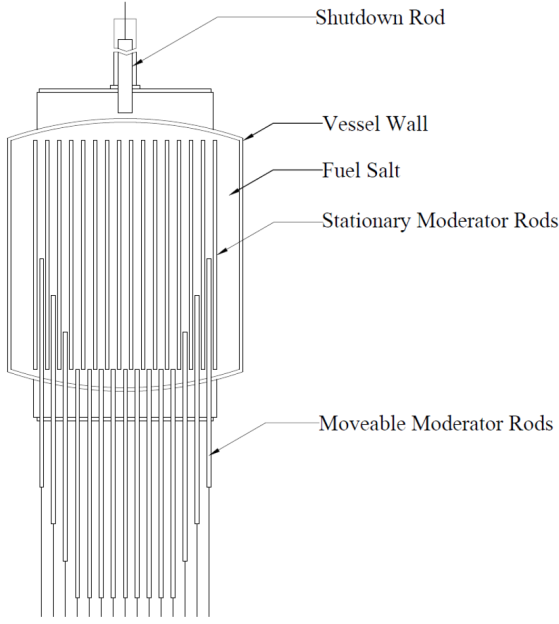
\includegraphics[width=0.55\textwidth]{tap_front_view.png}
  \caption{\gls{TAP} \gls{MSR} schematic view showing movable moderator rod 
  bundles and shutdown rod.}
  \label{fig:tap-main-view}
\end{figure}

\subsection{SERPENT 2 model} \label{sec:tap_model}
Advanced geometry surfaces and transformation capabilities of SERPENT are employed 
to represent \gls{TAP} core. 
Figure~\ref{fig:tap-serpent-plan} shows the plan view of preliminary whole-core
configuration at the expected reactor operational level when all
control rods are fully withdrawn. Figure~\ref{fig:tap-serpent-elev} shows the 
longitudinal section of the reactor. This model contains the moderator rods (with 
silicon carbide cladding), pressure vessel, and inlet and outlet plenums 
(Table~\ref{tab:tap_model_param}). The control rod cluster is made using 
\textbf{TRANS} SERPENT 2 feature which allows easy change control rod position 
during burnup simulations if necessary. The violet color represents zirconium 
hydride, and the yellow represents fuel 
salt. The blue color shows Hastelloy-N, a material used for the vessel wall, 
and the white color is a air. 
In this proposal, all figures of the core 
were generated using the built-in SERPENT plotter.
%%%%%%%%%%%%%%%%%%%%%%%%%%%%%%%%%%%%%%%%%%%%%%%%%%
\begin{table}[h!]
        \caption{Geometric parameters for the full-core 3D model of \gls{TAP} (reproduced from \cite{betzler_assessment_2017}). }
          \centering
        \begin{tabularx}{0.5\textwidth}{m x}
        \hline
         \qquad \textbf{Parameter}        			& 			             \\ \hline
         \quad \textit{Moderator rod}          		& 			 			 \\ 
         Cladding thickness, cm      	  			& 0.10     				 \\  
         Radius, cm				      	  			& 1.15     				 \\  
         Length, cm				      	  			& 300.0    				 \\  
         Pitch, cm				      	  			& 3.0    				 \\ \hline 
         \quad \textit{Moderator assemblies}   		& 			 			 \\ 
         Array					      	  			& 5 $\times$ 5			 \\  
         Pitch, cm				      	  			& 15.0    				 \\  \hline
         \quad \textit{Core}		          		& 			 			 \\ 
         Assemblies   				   	  			& 268     				 \\  
         Inner radius, cm		      	  			& 150.0    				 \\  
         Plenum height, cm			   	  			& 25.0    				 \\  
         Vessel wall thickness, cm     	  			& 5.0    				 \\             
         \hline
        \end{tabularx}
        \label{tab:tap_model_param}
\end{table}
%%%%%%%%%%%%%%%%%%%%%%%%%%%%%%%%%%%%%%%%%%%%%%%%
\begin{figure}[htp!] % replace 't' with 'b' to 
  \centering
		  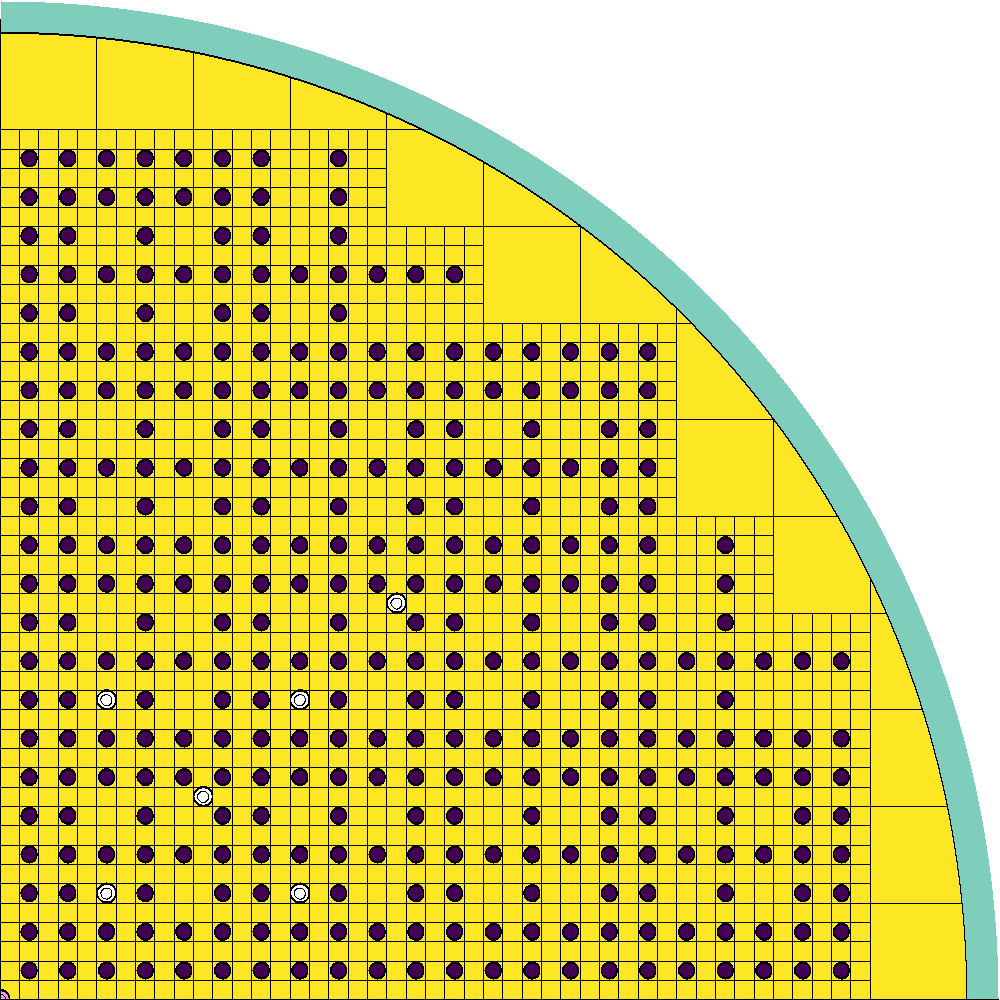
\includegraphics[width=\textwidth]{tap_plan_view.png}
  \caption{Plan view of SERPENT 2 \gls{TAP} model with fully withdrawn control rods.}
  \label{fig:tap-serpent-plan}
\end{figure}
\begin{figure}[htp!] % replace 't' with 'b' to 
  \centering
		  
\includegraphics[width=\textwidth]{tap_elev_view.png}
  \caption{Elevation view of SERPENT 2 \gls{TAP} model.}
  \label{fig:tap-serpent-elev}
\end{figure}

\subsection{TAP reprocessing system structure and simulation approach}
The \gls{TAP} nuclear island contains \gls{FP} removal system. Gaseous \glspl{FP} are 
continuously removed using off-gas system while liquid and solid \glspl{FP} are extracted 
via chemical processing system. As these byproducts are gradually removed, a small quantity 
of fresh fuel salt is regularly added to the primary loop. This process conserves a 
constant fuel salt mass and keeps the reactor critical. In contrast with \gls{MSBR} 
reprocessing system, \gls{TAP} does not need protactinium separation and isolation 
system because it operates in uranium-based single-stage fuel cycle. The authors of 
\gls{TAP} concept suggested three distinct fission product removal methods: 
\begin{enumerate}
	\item \textbf{Off-Gas System} removes gaseous fission products such as krypton 
and xenon, 
which are then compressed and stored temporarily until they have decayed to background 
radiation level. Trace amounts of tritium are also removed and bottled in a liquid form 
via the same process. In addition, the off-gas system also directly removes a small 
fraction of the noble metals.
	\item \textbf{Metal Plate-Out/Filtration} removes noble and semi-noble metal 
solid fission 
products as they plate out onto a nickel mesh filter located in a side stream in the 
primary loop.
	\item \textbf{Liquid Metal Extraction} separates lanthanides and other non-noble 
metals which 
remain primarily dissolved in the fuel salt. They generally have a lower capture cross 
section and thus absorb fewer neutrons than $^{135}$Xe but their extraction is essential 
to ensuring normal operation. In the \gls{TAP} lanthanides removal accomplishes via 
a liquid-metal/molten salt extraction process similar to one developed for \gls{MSBR} 
by \gls{ORNL} \cite{robertson_conceptual_1971} and discussed in Chapter 3. The process 
converts the dissolved lanthanides into a well-understood oxide waste form, similar to 
that of \gls{LWR} \gls{SNF}. This oxide waste comes out of the \gls{TAP} reprocessing 
plant in ceramic granules and can be sintered into another convenient form for storage.
\end{enumerate}

Table~\ref{tab:tap_reproc_methods} illustrates production rates and removal process for major fission products generate per year by one 520 MW$_e$ power plant.
%%%%%%%%%%%%%%%%%%%%%%%%%%%%%%%%%%%%%%%%%%%%%%%%%%
\begin{table}[h!]
        \caption{Fission product removal methods and approximate average production rate for \gls{TAP} operating at 100\% power level (reproduced from 
        \cite{transatomic_power_corporation_technical_2016}). }
          \centering
        \begin{tabularx}{\textwidth}{m s x x}
        \hline
\textbf{Fission Product}	& \textbf{Removal process} & \textbf{Production rate} & \textbf{Waste form}         \\
\hline
Noble gases ($^3$H, Kr, Xe) & Helium sparging & 100 kg/year     & Compressed gas     \\
\hline
Noble metals (Zn, Ga, Ge, As, Se, Nb, Mo, Tc, Ru, Rh, Pd, Ag, Cd, In, Sn, Sb, Te, I)									& Filtration and helium sparging & 200 kg/year     & Metallic\\
\hline
Lanthanides and others (Cr, Fe, Ni, Rb, Sr, Y, Zr, Cs, Ba, La, Ce, Pr,Nd, Pm, Sm, Eu, Gd, Tb, Dy, Ho, Er)             & Molten salt/liquid metal extraction        & 200 kg/year & Solid oxides \\
         \hline
        \end{tabularx}
        \label{tab:tap_reproc_methods}
\end{table}
%%%%%%%%%%%%%%%%%%%%%%%%%%%%%%%%%%%%%%%%%%%%%%%%
Figure~\ref{fig:tap-reproc} shows principal design of \gls{TAP} primary loop including 
off-gas system, nickel mesh filter, and lanthanides extraction chemical facility.
Overall, proposed fuel salt reprocessing approach is similar to one for \gls{MSBR} 
discussed in Chapter 3. Particularly, off-gas system also based on simple process of 
helium sparging through fuel salt with consequent gas bubbles removal before returning 
fuel salt back to the core. Nevertheless, one important difference must be noted: 
\gls{MSBR} gas separation system suggested helium injection and subsequent 
transport of the voids throughout the primary loop including core at least 10 full 
loops \cite{robertson_conceptual_1971}. It is significant concert to safe, stable 
operation because increase of void fraction in the fuel salt when it enters back 
to the core 
would cause positive reactivity insertion. This drawback can be overcome by using 
effective gas separator for stripping helium/xenon bubbles before returning the 
salt back to primary loop (Figure~\ref{fig:tap-reproc}, blue block). An effective 
method for 
stripping gas from the salt using centrifugal forces was proposed by Gabbard \cite{gabbard_development_1974}. The gas bubbles in axial-flow centrifugal bubble 
separator would be driven toward the center-line by the radial pressure gradient 
developed where it is removed through takeoff ports. The gas 
separation efficiency through this method was demonstrated to be dependent on 
salt flow rate (which is limitation factor for in-line removal system) but 
can be as large as 95\%. Gas removal efficiency was measured for this method 
under a wide variety of conditions and culminated in following equation for 
gas removal efficiency ($\epsilon_{g}$) \cite{gabbard_development_1974}:
\begin{equation} \label{eq:gas_eff}
\epsilon_g = \frac{2116.8 Q_g}{X Q_e P_{\gamma} + 2116.8 Q_g}
\end{equation}
where $Q_g$ is gas injection rate, scfm; $Q_e$ is liquid flow rate, cfm; $X$ is 
void fraction; $P_{\gamma}$ is absolute pressure, psf. This correlation will 
be used to realistically model an online molten salt gas removal system using 
a Python toolkit, SaltProc, developed as a part of my dissertation.
\begin{figure}[htp!] % replace 't' with 'b' to 
  \centering
		  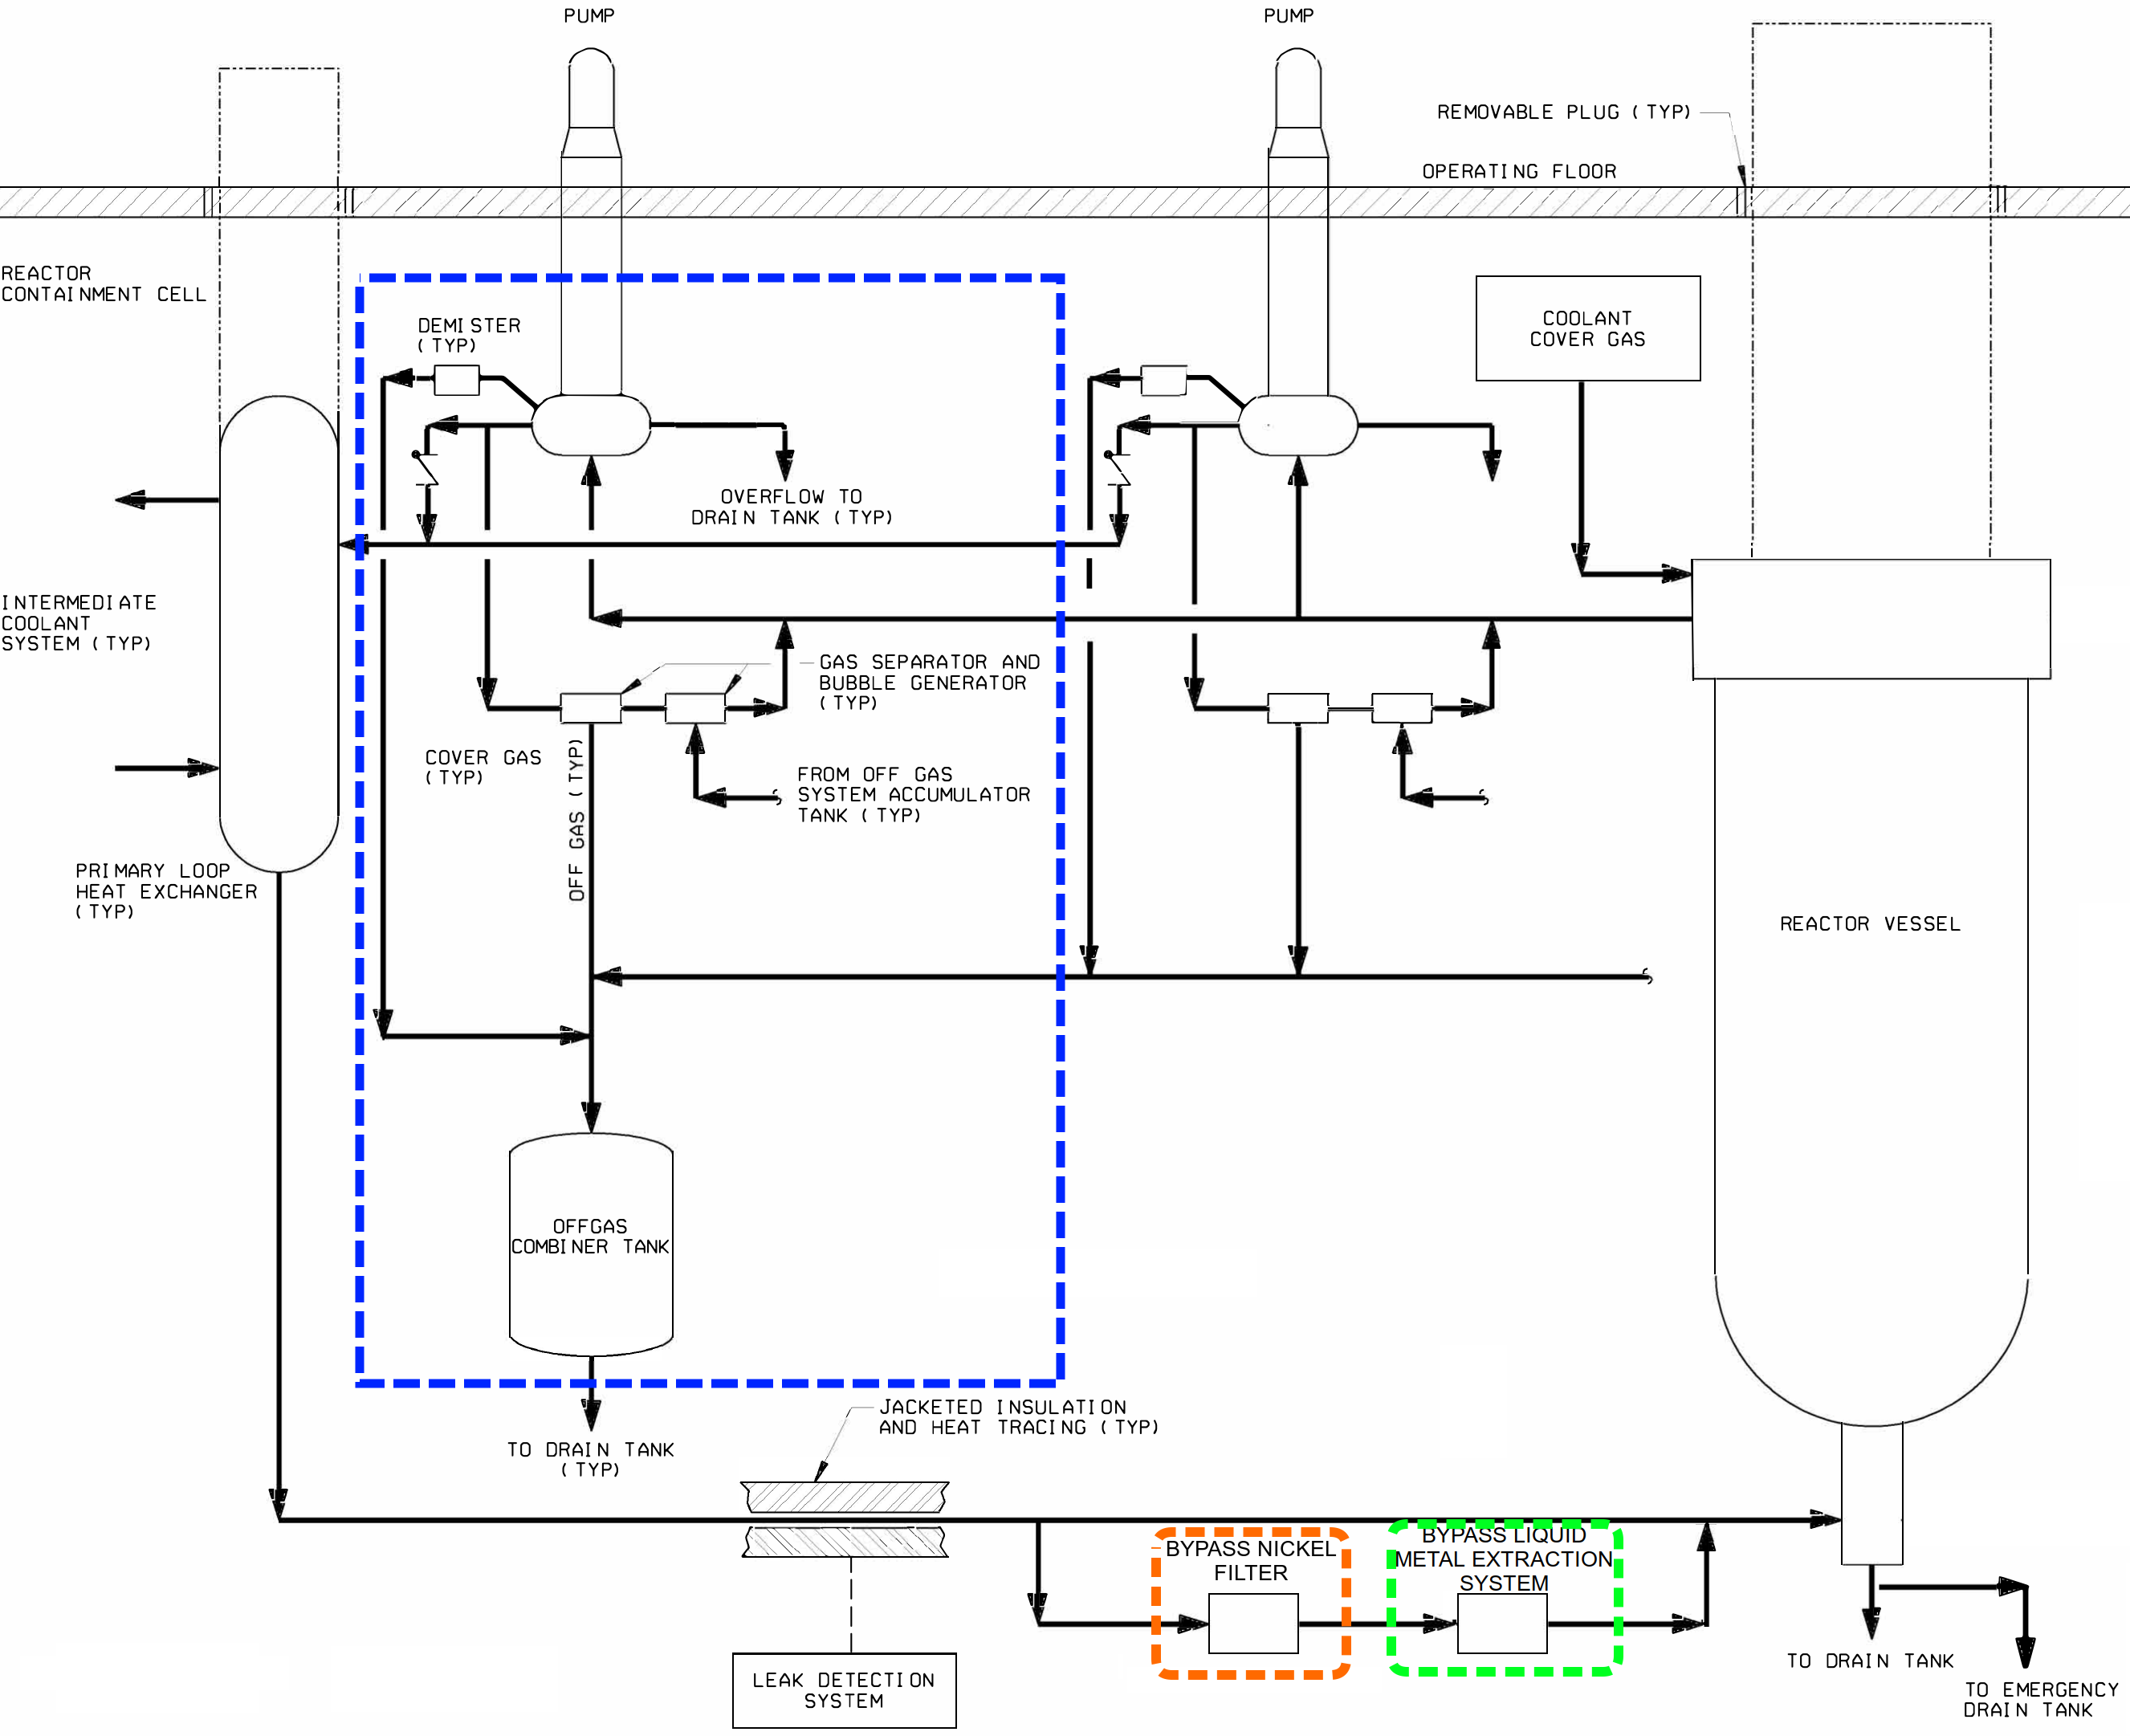
\includegraphics[width=\textwidth]{tap_primary_loop.png}
  \caption{Simplified \gls{TAP} primary loop design including off-gas system (blue), 
  nickel filter (orange) and liquid metal extraction system (green) (reproduced from \cite{transatomic_power_transatomic_2019}).}
  \label{fig:tap-reproc}
\end{figure}

Moreover, current research activity at University of Illinois at Urbana-Champaign 
``Enabling Load Following Capability in the Transatomic Power MSR" has a goal 
to obtain similar correlation for xenon removal efficiency for a prototypic 
gas stripping system using CFD modeling and set of small-scale experiments. This 
correlation will be also applied to \gls{TAP} depletion simulation to demonstrate capabilities of SaltProc tool to simulate realistic (rather than ideal 
\cite{transatomic_power_corporation_neutronics_2016, betzler_two-dimensional_2016,  betzler_assessment_2017}) \gls{TAP} 
system operation. In the same way, experimental and/or CFD correlations for gases 
removal efficiency will be valid for \gls{TAP}, \gls{MSBR} and any other \gls{MSR} 
(e.g. \gls{MSFR}) because these concepts uses FLi or FLiBe as fuel salt.

Noble and semi-noble metal solid fission products tends to plate out onto metal 
surfaces including piping, heat exchanger tubes, reactor vessel inner surface, etc. 
Previous research by \gls{ORNL} \cite{robertson_conceptual_1971} reported that 
about 50\% of noble and semi-noble metals would plate out inside \gls{MSBR} 
systems without any special treatment. To improve extraction efficiency for this 
fission products \gls{TAP} concept suggested employ a nickel mesh filter located 
in a bypass stream in the primary loop (Figure~\ref{fig:tap-reproc}, orange block). 
The main idea of this filter is to create large maze with large metal (nickel) 
surface area. The fuel salt flowing slowly through the filter and noble 
metals are accumulated on the filter surfaces. The removal efficiency 
($\epsilon_{noble}$) can be 
calculated as a function of the salt flow rate and filter interface area:
\begin{equation} \label{eq:filter_eff}
\epsilon_{noble} = F(\dot{m}_{salt}, A_f) = \frac{a A_f}{b \dot{m}_{salt} + c A_f}
\end{equation}
where $\dot{m}_{salt}$ is fuel salt mass flow rate; $A_f$ is the filter inner 
surface area (filter sizes and mesh pitch can be used to determine it); 
$a, b, c$ are correlation coefficients. This form of correlation will be used 
to inform online reprocessing model in SaltProc Python tool.

Liquid Metal Extraction process for \gls{TAP} concept has been taken from 
\gls{MSBR} which was discussed in sections~\ref{sec:chemical_processing} and \ref{sec:rare_earth_eff}. Removal efficiency ($\epsilon_{RE}$) of this process is function 
of fuel salt mass flow rate, liquid bismuth mass flow rate, interfacial areas 
between salt and metal, and mass transfer coefficient. The most recent 
research for LiF salt (for \gls{MSFR} concept) reported following form of 
extraction efficiency correlation \cite{rodrigues_actinide/lanthanide_2015}:
\begin{equation} \label{eq:re_eff}
\epsilon_{RE} = \frac{1}{1+10^{\lambda}} = \frac{1}{1+10^{f(A, \dot{m}_{Bi}, \dot{m}_{salt}, N, K)}}
\end{equation}
where $A$ is a metal-to-salt interface area, $\dot{m}_{Bi}$ is bismuth mass 
flow rate, $\dot{m}_{salt}$ is salt mass flow rate, $N$ is the number of stages, 
$K$ is mass transfer coefficient at the salt / Bi-Li interface. Correlations are 
different for various lanthanides and can be determined from experimental data 
and/or existing analytical models \cite{mcneese_engineering_1971, simon_-line_2008, rodrigues_actinide/lanthanide_2015, delpech_reactor_2009, delpech_possible_2012}.

In fact, due to similarities in reprocessing schemes, \gls{TAP} project reported almost 
the same set of elements for removal and similar effective cycle times as was suggested 
for \gls{MSBR} (Table~\ref{tab:reprocessing_list}). The \gls{TAP} neutronics whitepaper 
specifies additional low-probability fission products and gases that should be 
removed during operation. These elements are categorized into the previously 
defined processing groups, but the removal rates of most of these elements 
(i.e., all except for hydrogen) are very low.
%%%%%%%%%%%%%%%%%%%%%%%%%%%%%%%%%%%%%%%%
\begin{table}[ht!]
        \centering
        \caption{The effective cycle times for fission products removal (reproduced from \cite{betzler_implementation_2017}).}
        \begin{tabular}{p{0.25\textwidth} p{0.45\textwidth} p{0.16\textwidth}}
        \hline 
        %\begin{tabularx}{\linewidth}{l X} \toprule 
        Processing group & \qquad\qquad\qquad Nuclides & Cycle time (at full power) \\ [5pt] \hline 
 \multicolumn{3}{c}{\textit{Elements removed in \gls{MSBR} concept and adopted for \gls{TAP}} \cite{robertson_conceptual_1971, rykhlevskii_modeling_2019}} \\
        Volatile gases & Xe, Kr								  & 20 sec \\ [5pt]
        Noble metals & Se, Nb, Mo, Tc, Ru, Rh, Pd, Ag, Sb, Te & 20 sec \\ [5pt]
        Seminoble metals & Zr, Cd, In, Sn	  				  & 200 days \\ [5pt]
        Volatile fluorides & Br, I 							  & 60 days \\ [5pt]
        Rare earths & Y, La, Ce, Pr, Nd, Pm, Sm, Gd & 50 days \\ [5pt]
        \qquad & Eu & 500 days \\ [5pt]
        Discard & Rb, Sr, Cs, Ba & 3435 days \\ [5pt] 
        \hline
 
 \multicolumn{3}{c}{\textit{Additional elements removed} \cite{transatomic_power_corporation_neutronics_2016}  } \\
        Volatile gases & H								  		& 20 sec    \\ [5pt]
        Noble metals & Ti, V, Cr, Cu						    & 3435 days \\ [5pt]
        Seminoble metals & Mn, Fe, Co, Ni, Zn, Ga, Ge, As       & 3435 days \\ [5pt]
        Rare earths & Sc										& 3435 days \\ [5pt]
        Discard & Ca											& 3435 days \\ [5pt] 
        \hline
        \end{tabular}
        \label{tab:reprocessing_list}
          \vspace{-0.9em}
\end{table}

Details of gas removal and fuel reprocessing systems have historically been conceptual 
and liquid-fueled system designers including \gls{TAP} usually assumes ideal (rather 
than realistically constrained) removal efficiencies for reactor performance simulations.
Based on detailed data from this section (Table~\ref{tab:reprocessing_list}) and 
correlations~\ref{eq:gas_eff},\ref{eq:filter_eff},\ref{eq:re_eff} the realistic 
online reprocessing system and reactor model will be created to capture the dynamics 
of fuel composition evolution during reactor operation.


\section{Preliminary results}
The ability of liquid-fueled systems to continuously remove fission products and add 
fissile and/or fertile elements is the main challenge for depletion simulations. 
First version of SaltProc takes into account online separations and feeds using the 
SERPENT 2 continuous-energy Monte Carlo neutron transport and depletion code 
\cite{rykhlevskii_arfc/saltproc_2018}. Developed as a part of master thesis, this 
version of tool only able to leverage ideal 
removals (e.g., 100\% of target isotope mass extracted). Capabilities of this tool 
has been demonstrated for full-core \gls{MSBR} model \cite{rykhlevskii_modeling_2019}. 
Key findings from this effort are presented in section~\ref{sec:msbr_reproc}.

Additionally to high-precision whole-core \gls{MSBR} model, as a part of 
proposed dissertation research, full-core model of 
\gls{TAP} \gls{MSR} (section~\ref{sec:tap_model}) was developed to 
demonstrate SaltProc capabilities and cross-verify it against previous research.

\subsection{MSBR online reprocessing analysis} \label{sec:msbr_reproc}
The \gls{MSBR} vessel has a diameter of 680 cm and a height of 610 cm. It 
contains a molten fluoride fuel-salt mixture that generates heat in the active 
core region and transports that heat to the primary heat exchanger by way of 
the primary salt pump. In the active core region, the fuel salt flows through 
channels in moderating and reflecting graphite blocks. 
Figure~\ref{fig:serpent_plan_view} shows the configuration of the 
\gls{MSBR} vessel, including the ``fission" (zone I) and ``breeding" 
(zone II) regions inside the vessel. The core has two radial zones bounded by a 
solid cylindrical graphite reflector and the vessel wall. The central zone, 
zone I, in which 13\% of the volume is fuel salt and 87\% graphite, is
composed of 1,320 graphite cells, 2 graphite control rods, and 2 
safety\footnote{ These rods needed for emergency shutdown only.} rods. The 
under-moderated zone, zone II, with 37\% fuel salt, and radial reflector, 
surrounds the zone I core region and serves to diminish neutron leakage. Zones 
I and II are surrounded radially and axially by fuel salt 
(figure~\ref{fig:serpent_zoneII}). This space for fuel is necessary for 
injection and flow of molten salt.
\begin{figure}[hbp!] % replace 't' with 'b' to \centering
  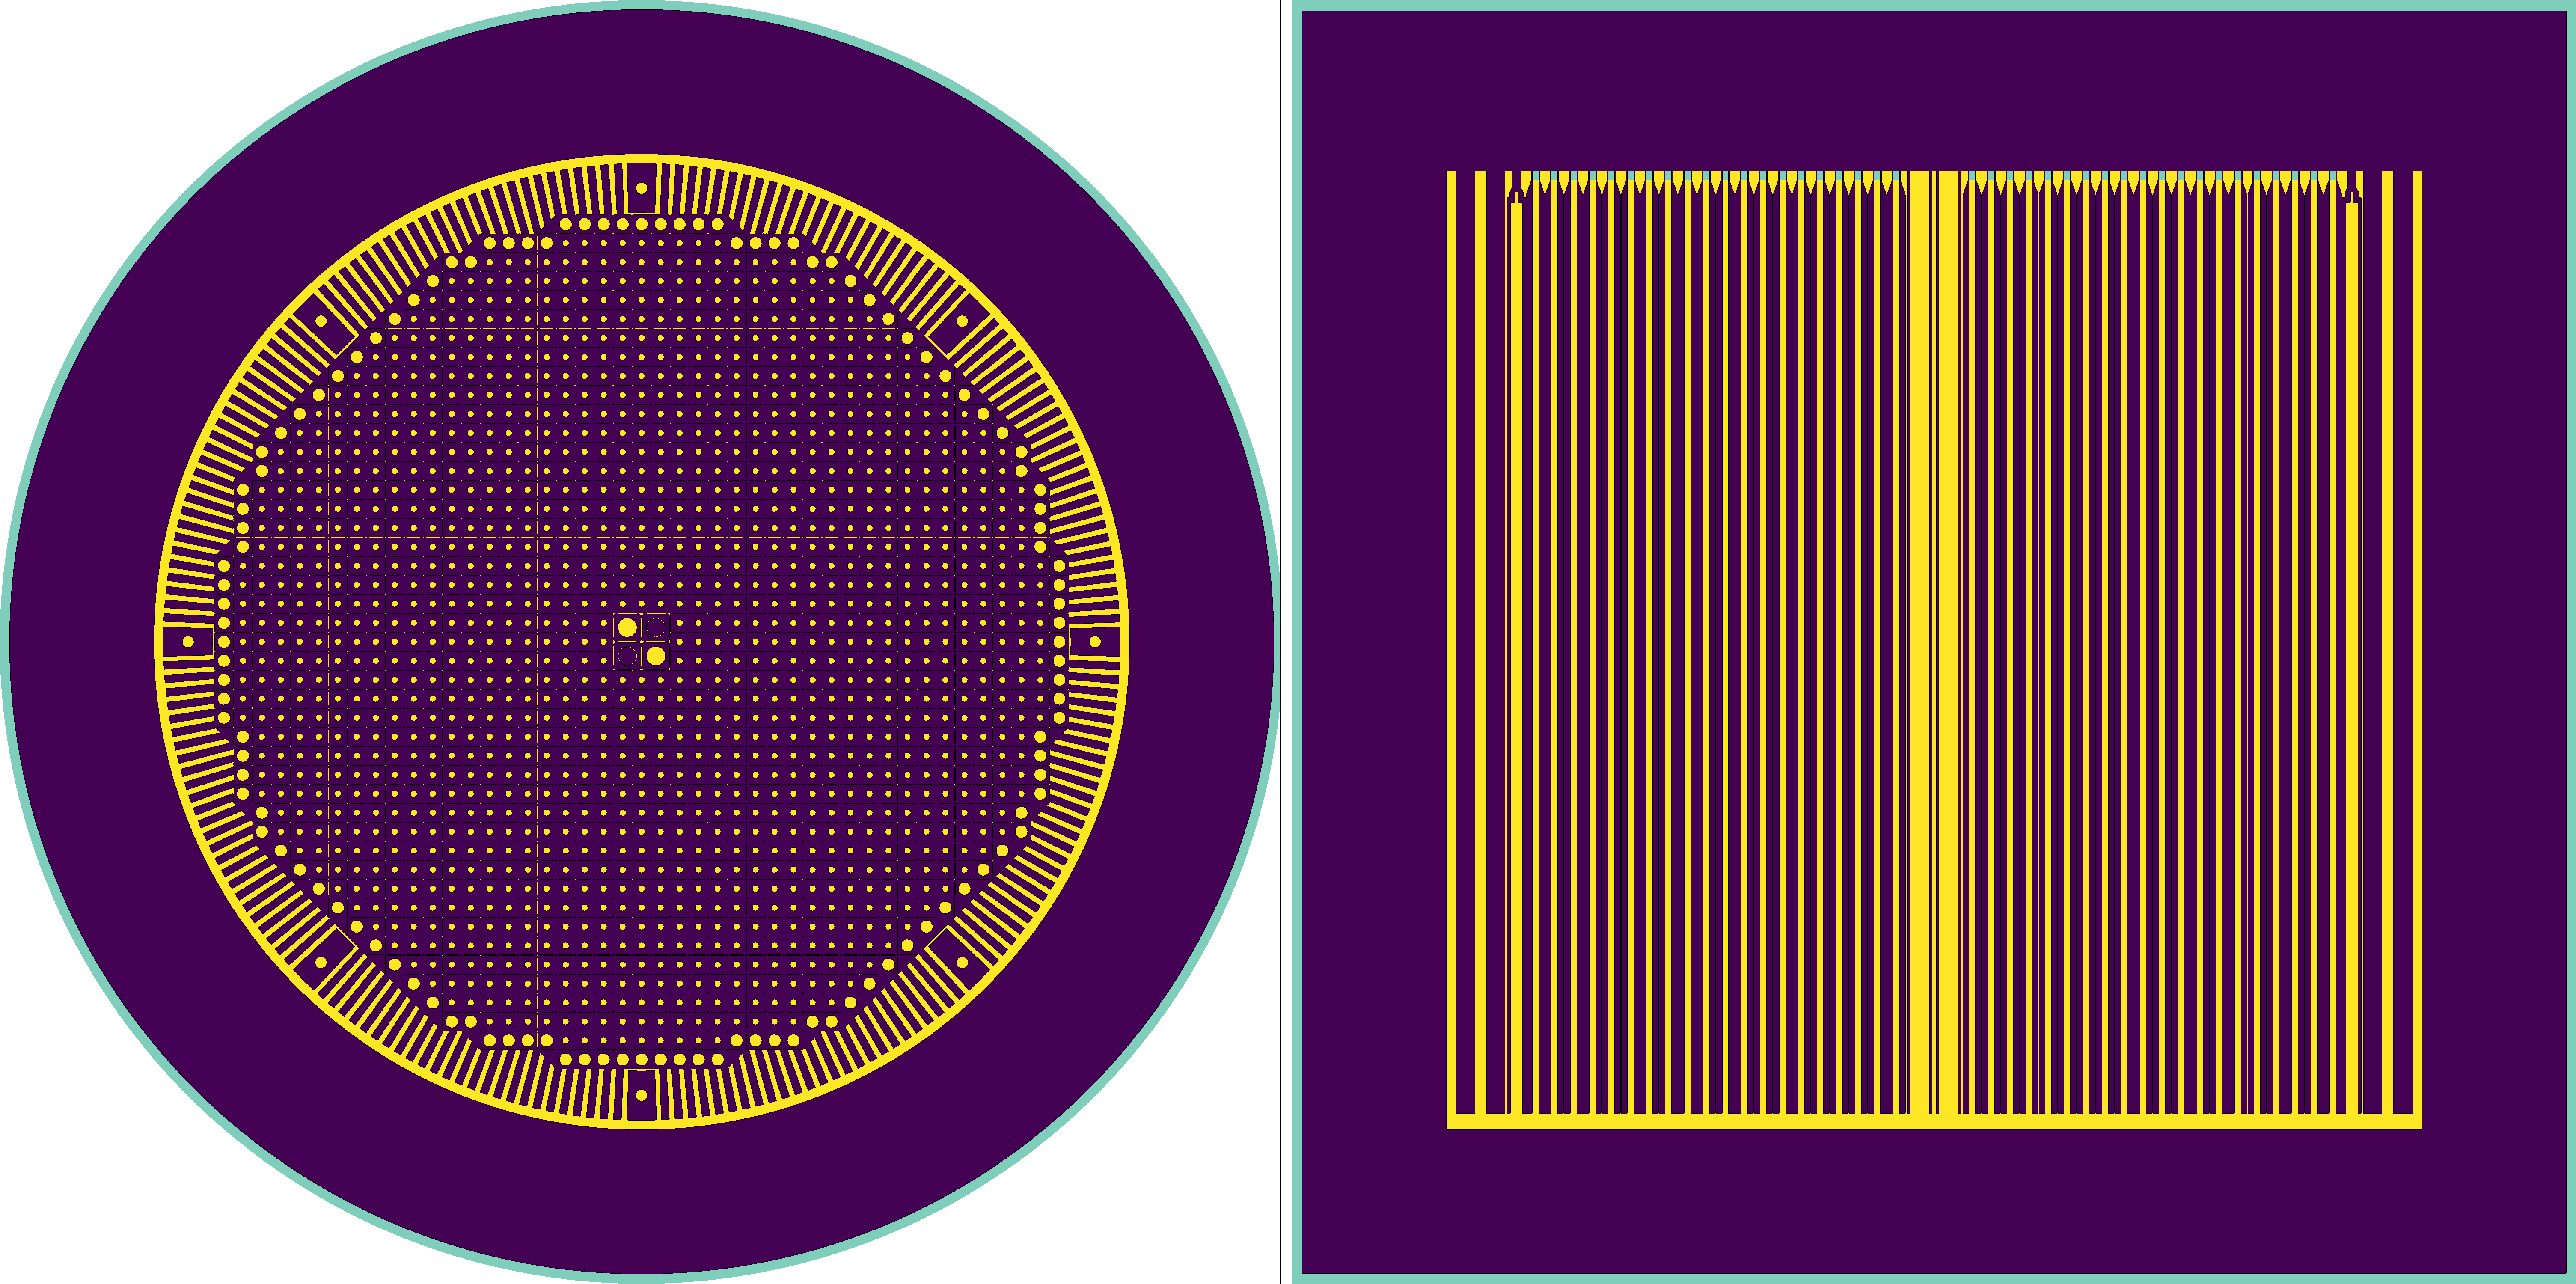
\includegraphics[width=\textwidth]{view_serpent.png}
  \caption{Plan and elevation views of SERPENT 2 \gls{MSBR} model developed in 
  this work.}
  \label{fig:serpent_plan_view}
\end{figure}
\begin{figure}[t!] % replace 't' with 'b' to \centering
  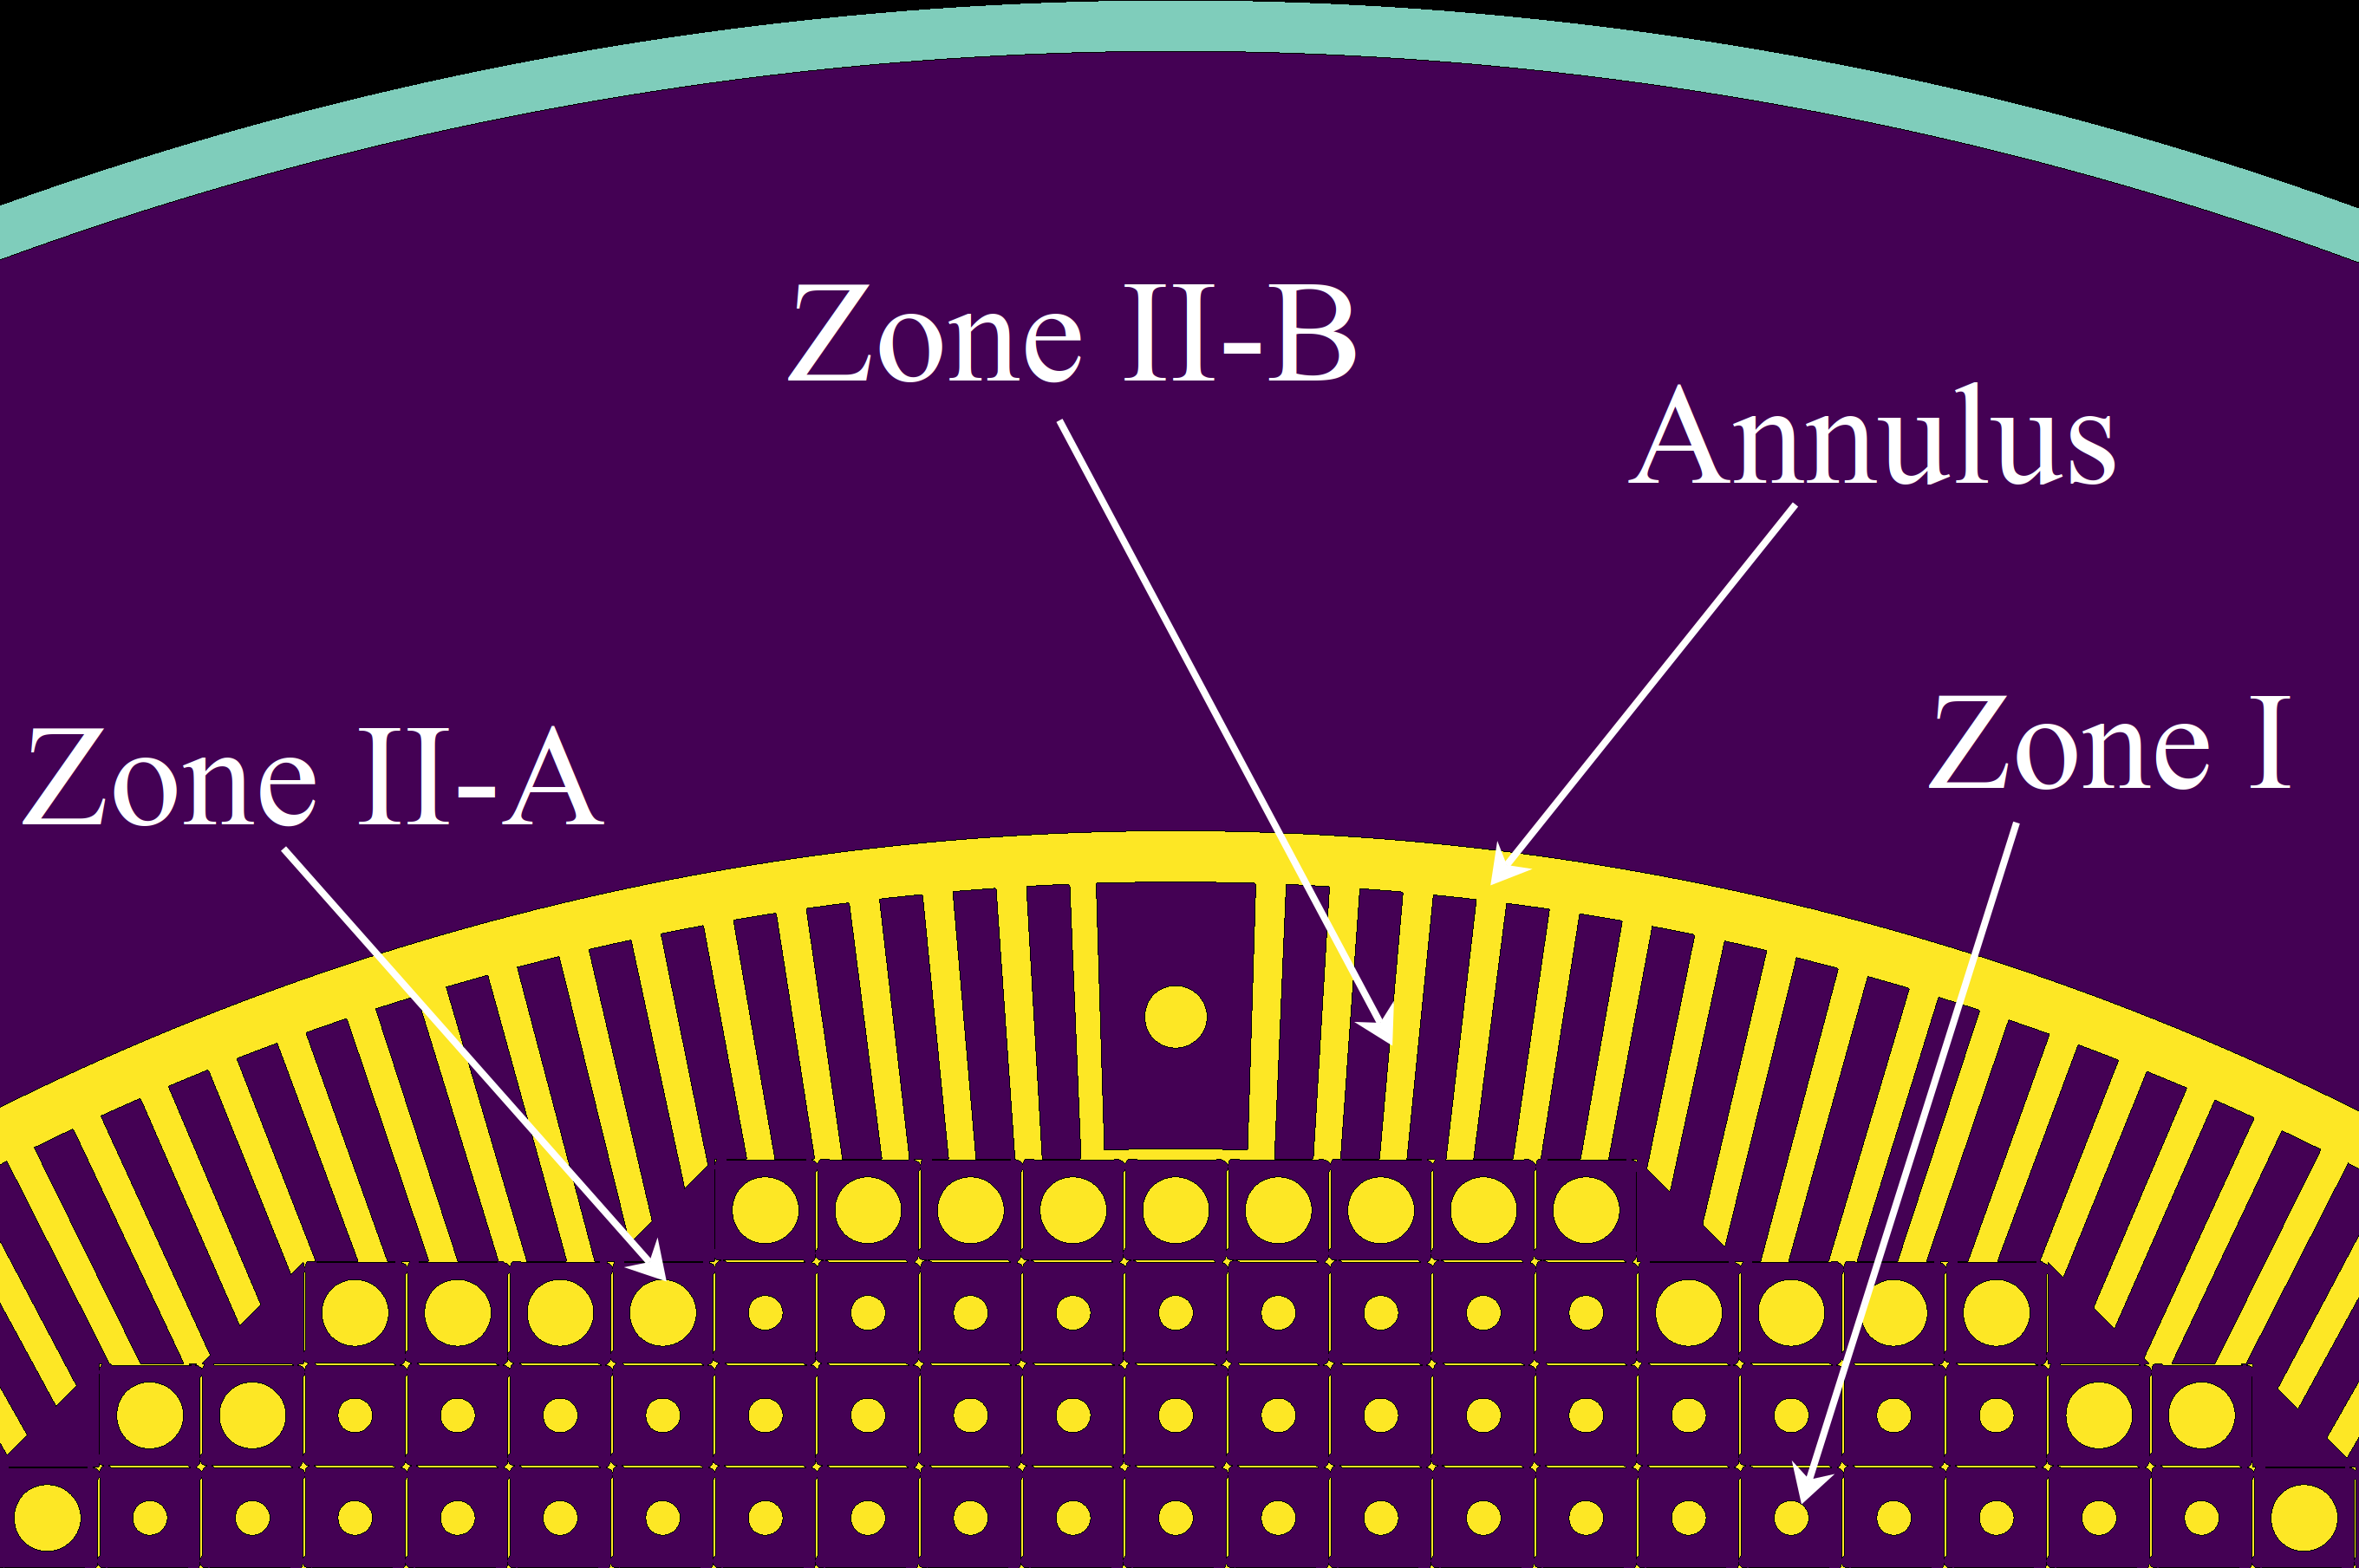
\includegraphics[width=\textwidth]{ser_zone_II.png}
  \caption{Detailed view of \gls{MSBR} two zone model. 
          Yellow represents fuel salt, purple represents graphite, and aqua represents the reactor vessel.}
  \label{fig:serpent_zoneII}
\end{figure}

The $^{232}$Th in the fuel absorbs thermal neutrons and produces $^{233}$Pa 
which then decays into the fissile $^{233}$U. Furthermore, the \gls{MSBR} 
design requires online reprocessing to remove all poisons (e.g. $^{135}$Xe), 
noble metals, and gases (e.g. $^{75}$Se, $^{85}$Kr) every 20 seconds. 
Protactinium presents a challenge, since it has a large absorption cross 
section in the thermal energy spectrum. Moreover, $^{233}$Pa left in the core
would produce $^{234}$Pa and $^{234}$U, neither of which are useful as fuel. 
Accordingly, $^{233}$Pa is continuously 
removed from the fuel salt into a protactinium decay tank to allow $^{233}$Pa 
to decay to $^{233}$U without the corresponding negative neutronic impact. The reactor 
reprocessing system must separate $^{233}$Pa from the molten-salt fuel over 3 
days, hold it while $^{233}$Pa decays into $^{233}$U, and return it back to the 
primary loop. This feature allows the reactor to avoid neutron losses to 
protactinium, lowers in-core fission product inventory, and increases the 
efficiency of $^{233}$U breeding. Upper part of table~\ref{tab:reprocessing_list} 
summarizes full list of nuclides and the ``cycle times''\footnote{ The \gls{MSBR} 
program defined a ``cycle time" as the amount of time required to remove 100\% of 
a target nuclide from a fuel 
salt \cite{robertson_conceptual_1971}.} used for modeling salt treatment and 
separations \cite{robertson_conceptual_1971}. 
The removal rates vary among nuclides in this reactor concept which dictate the 
necessary resolution of depletion calculations. If the depletion time intervals 
are very short, an enormous number of depletion steps are required to obtain 
the equilibrium composition. On the other hand, if the depletion  calculation 
time interval is too long, the impact of short-lived fission products is not 
captured. To compromise, a 3 day time interval was selected for depletion 
calculations to correlate with the removal interval of 
$^{233}$Pa and $^{232}$Th was continuously added to maintain the initial mass 
fraction of $^{232}$Th.

Figures~\ref{fig:keff}, \ref{fig:keff_zoomed} show the effective multiplication factors 
obtained using SaltProc and SERPENT2. The effective multiplication factors were 
calculated after removing fission products listed in 
Table~\ref{tab:reprocessing_list} and adding the fertile material at the end of 
cycle time (3 days for this work). The effective multiplication 
factor fluctuates significantly as a result of the batch-wise nature of this 
online reprocessing strategy. 
\begin{figure}[ht!] 
  \centering
  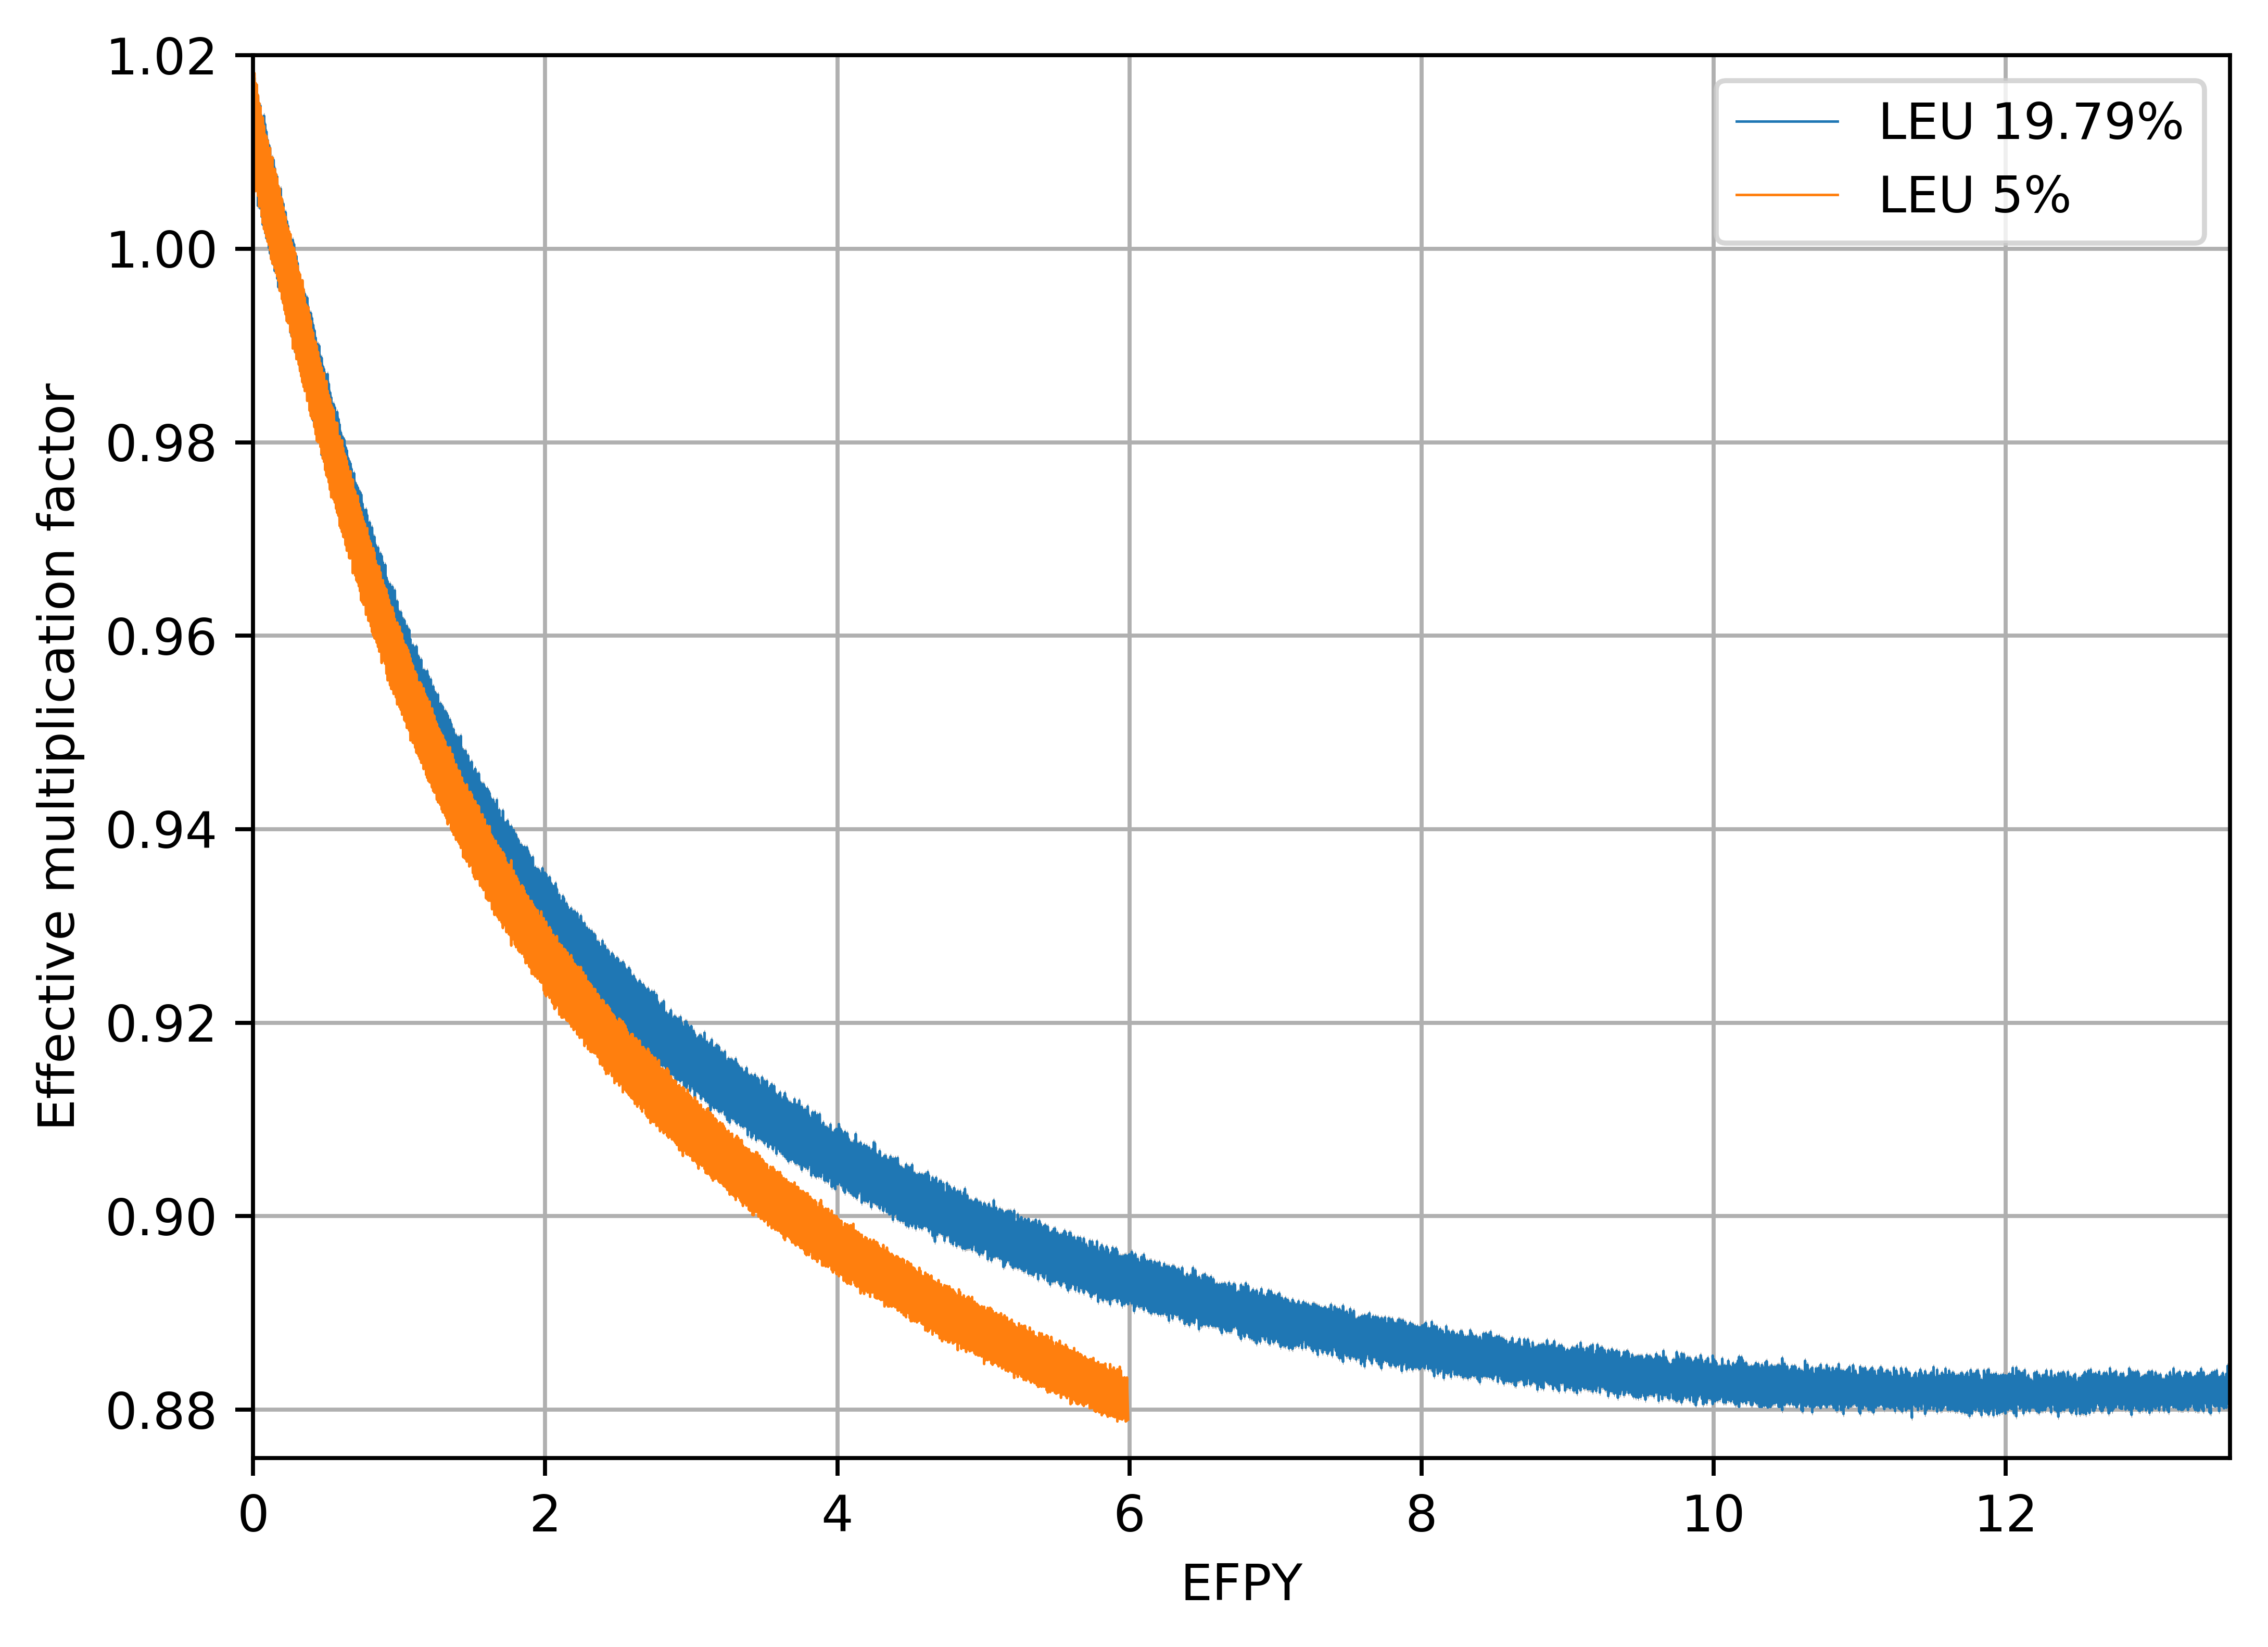
\includegraphics[width=\textwidth]{keff.png}
  \caption{Effective multiplication factor dynamics for full-core \gls{MSBR} 
  model over a 60-year reactor operation lifetime.}
  \label{fig:keff}
\end{figure}
\begin{figure}[ht!] 
  \centering
  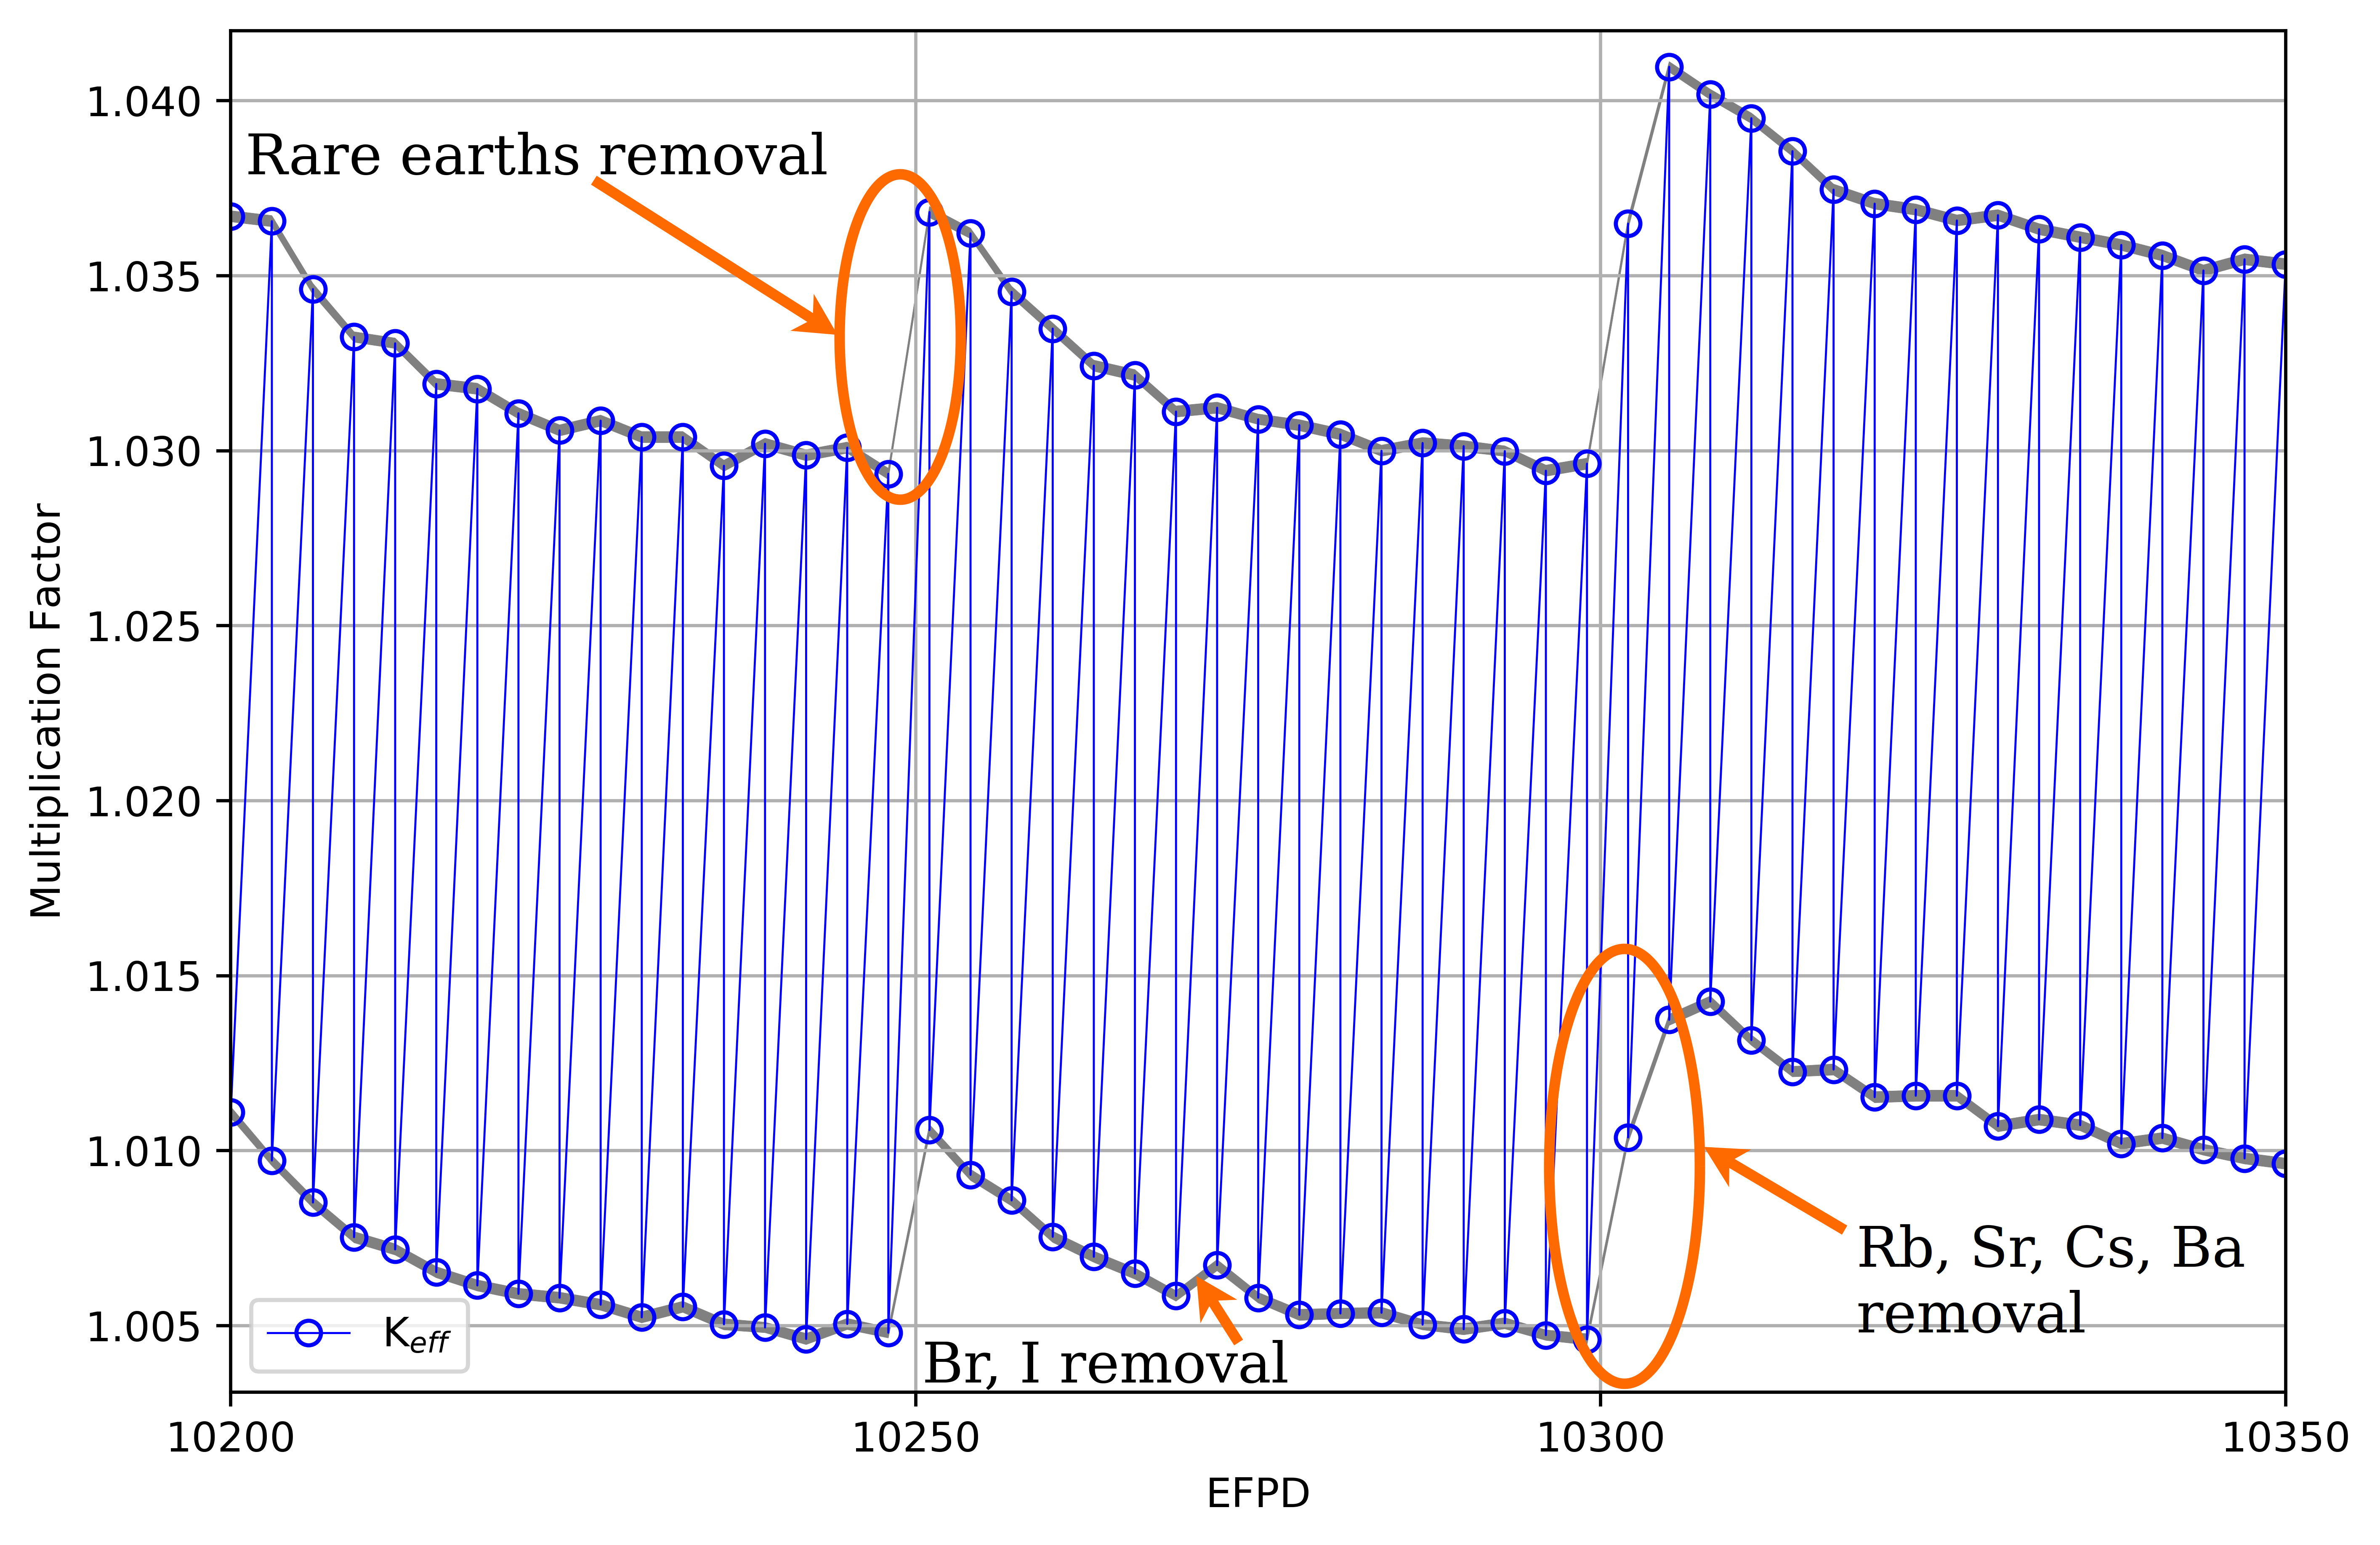
\includegraphics[width=\textwidth]{keff_zoomed.png}
  \caption{Zoomed effective multiplication factor for 150-EFPD time interval.}
  \label{fig:keff_zoomed}
\end{figure}

First, SERPENT calculates the effective multiplication factor for the beginning 
of the cycle (there is fresh fuel composition at the first step). Next, it 
computes the new fuel salt composition at the end of a 3-day depletion. The 
corresponding effective multiplication factor is much smaller than the previous 
one. Finally, SERPENT calculates $k_{eff}$ for the depleted composition after 
applying feeds and removals. The $K_{eff}$ increases accordingly since major reactor 
poisons (e.g. Xe, Kr) are removed, while fresh fissile material ($^{233}$U) 
from the protactinium decay tank is added.  

Additionally, the presence of rubidium, strontium, cesium, and barium in the 
core are disadvantageous to reactor physics. 
Overall, the effective multiplication factor gradually decreases from 1.075 to 
$\approx$1.02 at equilibrium after approximately 6 years of irradiation. 

Loading initial fuel salt composition into the \gls{MSBR} core leads to a 
supercritical configuration (Figure ~\ref{fig:fp_removal}). After reactor 
startup, the effective multiplication factor for the case with volatile gases 
and noble metals removal is approximately 7500 pcm  higher than for case with 
no fission products removal. This significant impact on the reactor core is
achieved due to immediate removal (20 sec cycle time) and high absorption cross 
section of Xe, Kr, Mo, and other noble metals removed. The effect of rare earth 
element removal is considerable a few months after startup and reached 
approximately 5500 pcm after 10 years of operation. The rare earth elements were 
removed at a slower rate (50-day cycle time). Moreover, 
Figure~\ref{fig:fp_removal} demonstrates that batch-wise removal of strong 
absorbers every 3 days did not necessarily leads to fluctuation in results 
but rare earth elements removal every 50 days causes an approximately 600 pcm jump 
in reactivity.

The effective multiplication factor of the core reduces gradually over 
operation time because the fissile material ($^{233}$U) continuously depletes 
from the fuel salt due to fission while fission products 
accumulate in the fuel salt simultaneously. Eventually, without fission products removal, 
the reactivity decreases to the subcritical state after approximately 500 and 
1300 days of operation for cases with no removal and volatile gases \& noble 
metals removal, respectively. The time when the simulated core reaches 
subcriticality ($k_{eff}<$1.0) for full-core model) is called the core lifetime. 
Therefore, removing fission products provides with significant neutronic benefit 
and enables a longer core lifetime.
\begin{figure}[ht!] % replace 't' with 'b' to force it to 
  \centering
  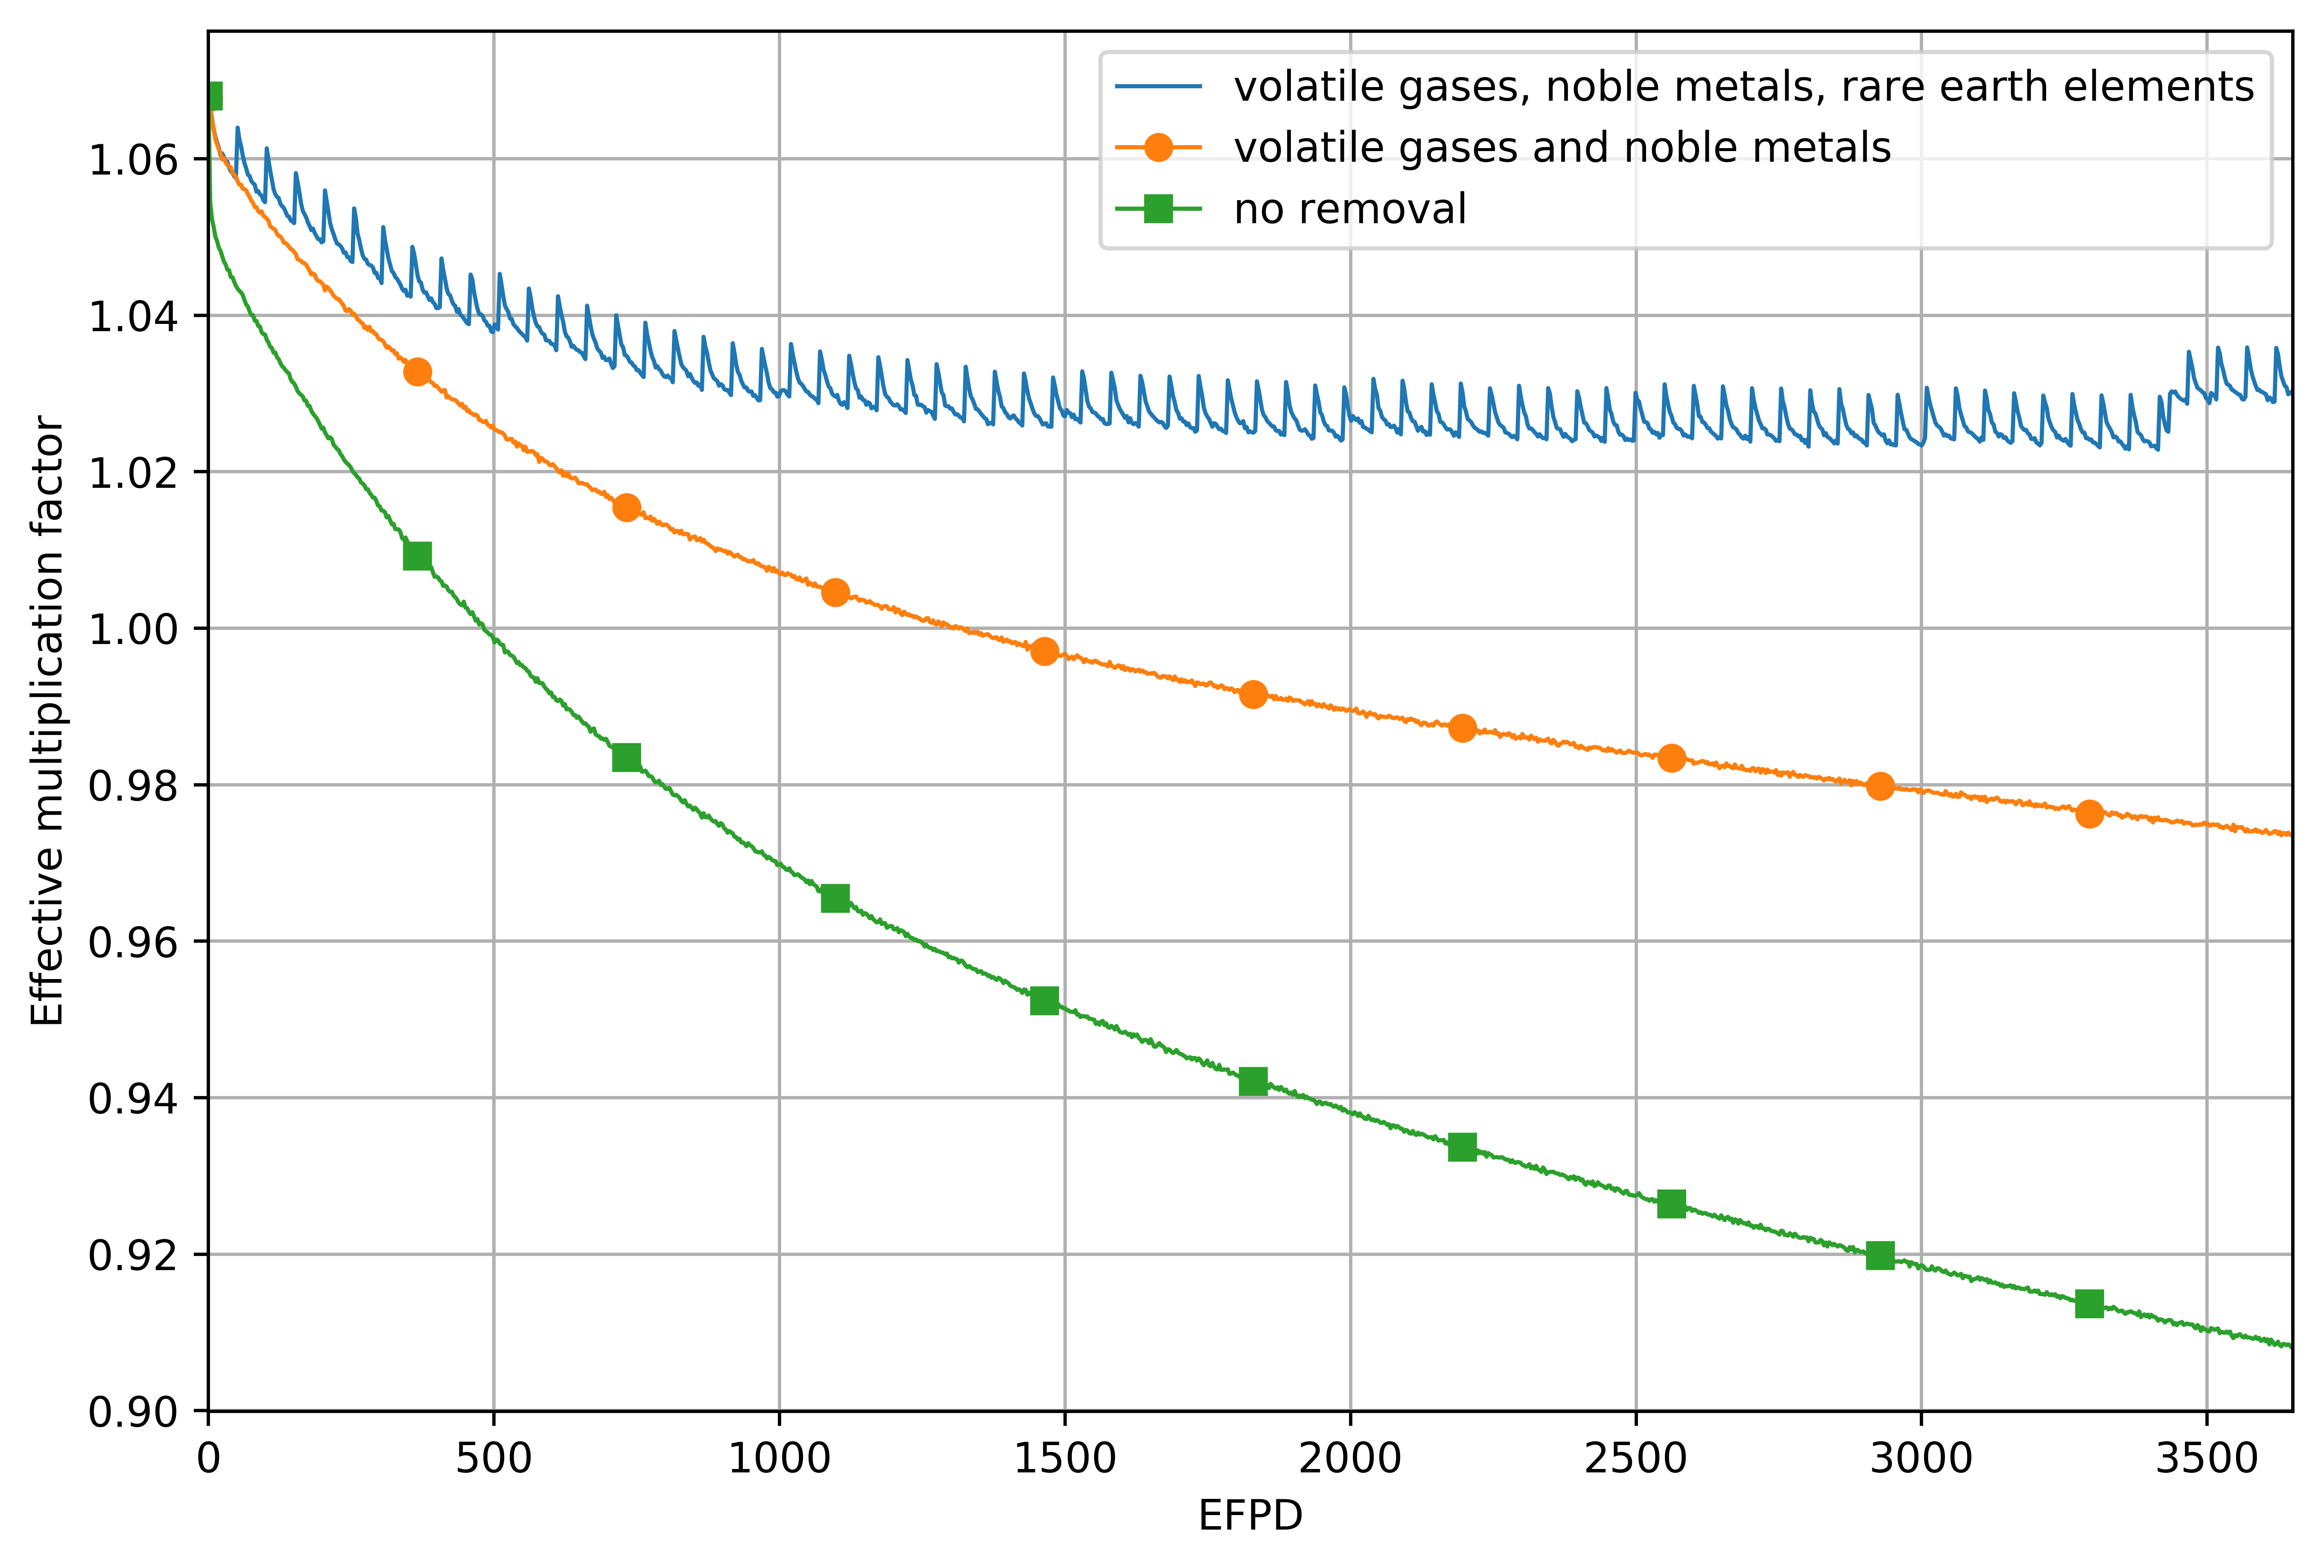
\includegraphics[width=\textwidth]{keff_rem_cases.png} 
  \caption{Calculated effective multiplication factor for full-core \gls{MSBR} 
model with removal of various fission product groups over 10 years of 
operation.}
  \label{fig:fp_removal}
\end{figure}

This preliminary results have been demonstrate SaltProc's capability to find 
the equilibrium fuel salt 
composition (where equilibrium is defined as when the number densities of major 
isotopes vary by less than 1\% over several years). Additionally this results
has been show benefits of continuous fission products removal for 
thermal \gls{MSR} design. Developed full-core high-fidelity benchmark model 
of the \gls{MSBR} will be employed for new version of SaltProc demonstration 
and validation. 